%==========================================================================

\begin{frame}[fragile]

  {\Huge Scratch memory}

  \vspace{20pt}

  \textbf{Learning objectives:}
  \begin{itemize}
    \item {Understand concept of \textbf{team} and \textbf{thread} private \textbf{scratch pads}}
    \item {Understand how scratch memory can \textbf{reduce global memory accesses}}
    \item {Recognize \textbf{when to use} scratch memory}
    \item {Understand \textbf{how to use} scratch memory and when barriers are necessary}
  \end{itemize}

  \vspace{-20pt}

\end{frame}

%==========================================================================

\begin{frame}[fragile]{Types of Scratch Space Uses}
\vspace{-8pt}
\textbf{Two Levels of Scratch Space}
\begin{itemize}
\item{Level 0 is limited in size but fast.}
\item{Level 1 allows larger allocations but is equivalent to High Bandwidth Memory in latency and bandwidth.}
\end{itemize}

\textbf{Team or Thread private memory}
\begin{itemize}
\item{Typically used for per work-item temporary storage.}
\item{Advantage over pre-allocated memory is aggregate size scales with number of threads, not number of work-items.}
\end{itemize}

\textbf{Manually Managed Cache}
\begin{itemize}
\item{Explicitly cache frequently used data.}
\item{Exposes hardware specific on-core scratch space (e.g. NVIDIA GPU Shared Memory).}
\end{itemize}

\pause
\vspace{2pt}
\textbf{Now: Discuss Manually Managed Cache Usecase.}
\end{frame}
%==========================================================================

\begin{frame}[fragile]{Example: contractDataFieldScalar (1)}

  \ul{\textbf{One slice of contractDataFieldScalar:}}

  \vspace{-10pt}

  \begin{center}
    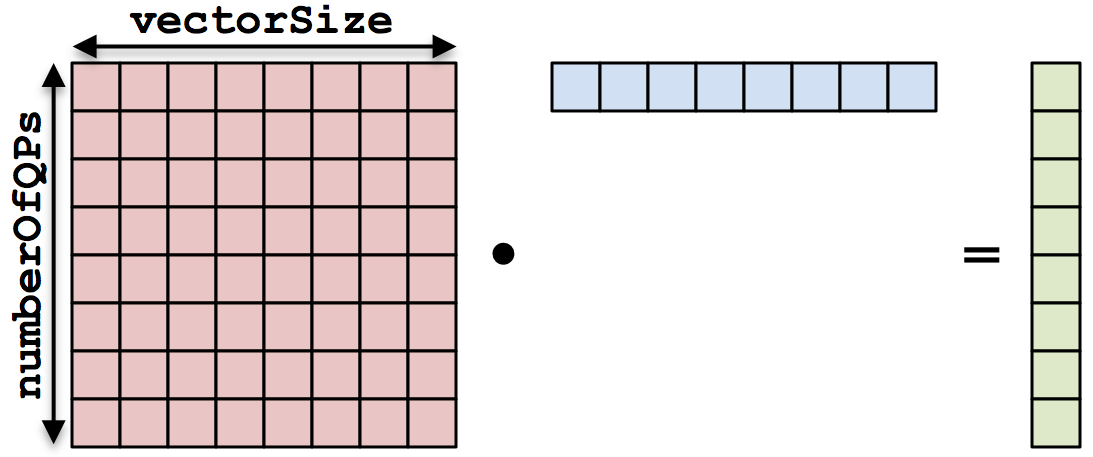
\includegraphics[width=0.65\textwidth]{figures/ContractDataFieldScalar_slice}
  \end{center}

  \begin{code}[frame=single, keywords={}]
for (qp = 0; qp < numberOfQPs; ++qp) {
  total = 0;
  for (i = 0; i < vectorSize; ++i) {
    total += @darkredA@darkred(qp, i) * @blueB@blue(i);
  }
  @darkgreenresult@darkgreen(qp) = total;
}
  \end{code}

\end{frame}

%==========================================================================

\begin{frame}[fragile]{Example: contractDataFieldScalar (2)}

  \ul{\textbf{contractDataFieldScalar:}}

  \vspace{-10pt}

  \begin{center}
    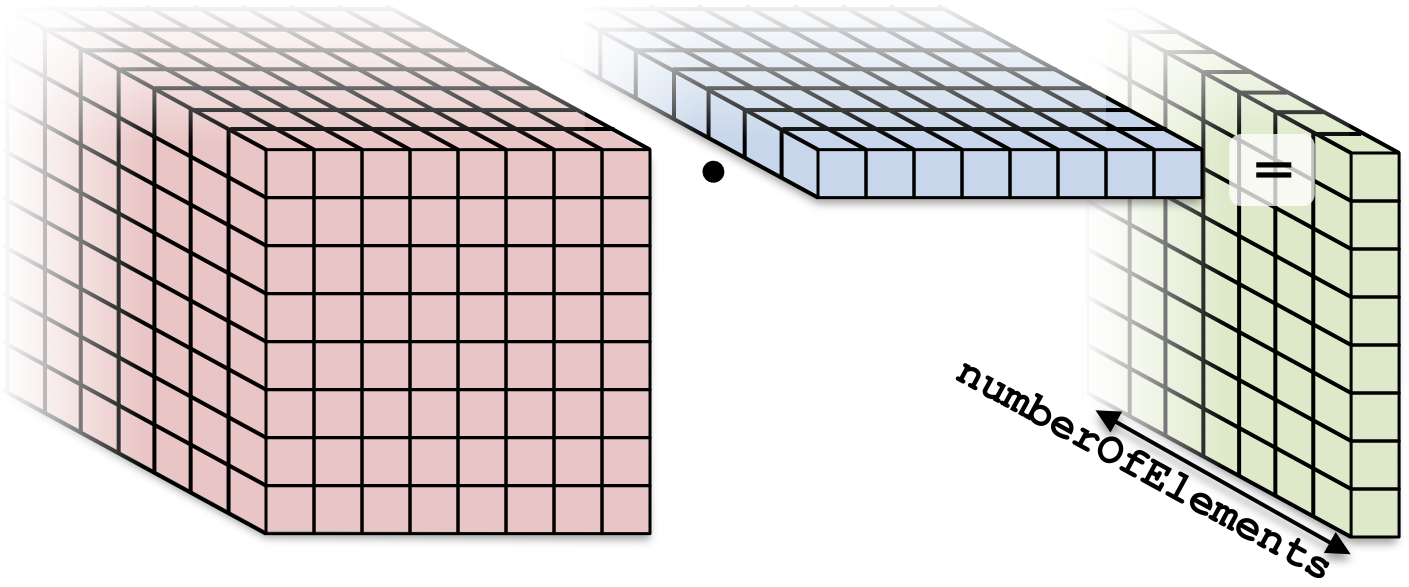
\includegraphics[width=0.75\textwidth]{figures/ContractDataFieldScalar}
  \end{center}

  \vspace{-10pt}

  \begin{code}[frame=single, keywords={}]
for (element = 0; element < numberOfElements; ++element) {
  for (qp = 0; qp < numberOfQPs; ++qp) {
    total = 0;
    for (i = 0; i < vectorSize; ++i) {
      total += @darkredA@darkred(element, qp, i) * @blueB@blue(element, i);
    }
    @darkgreenresult@darkgreen(element, qp) = total;
  }
}
  \end{code}

\end{frame}

%==========================================================================

\begin{frame}[fragile]{Example: contractDataFieldScalar (3)}

  \begin{columns}[t,onlytextwidth]
    \column{.55\textwidth}
      \begin{center}
        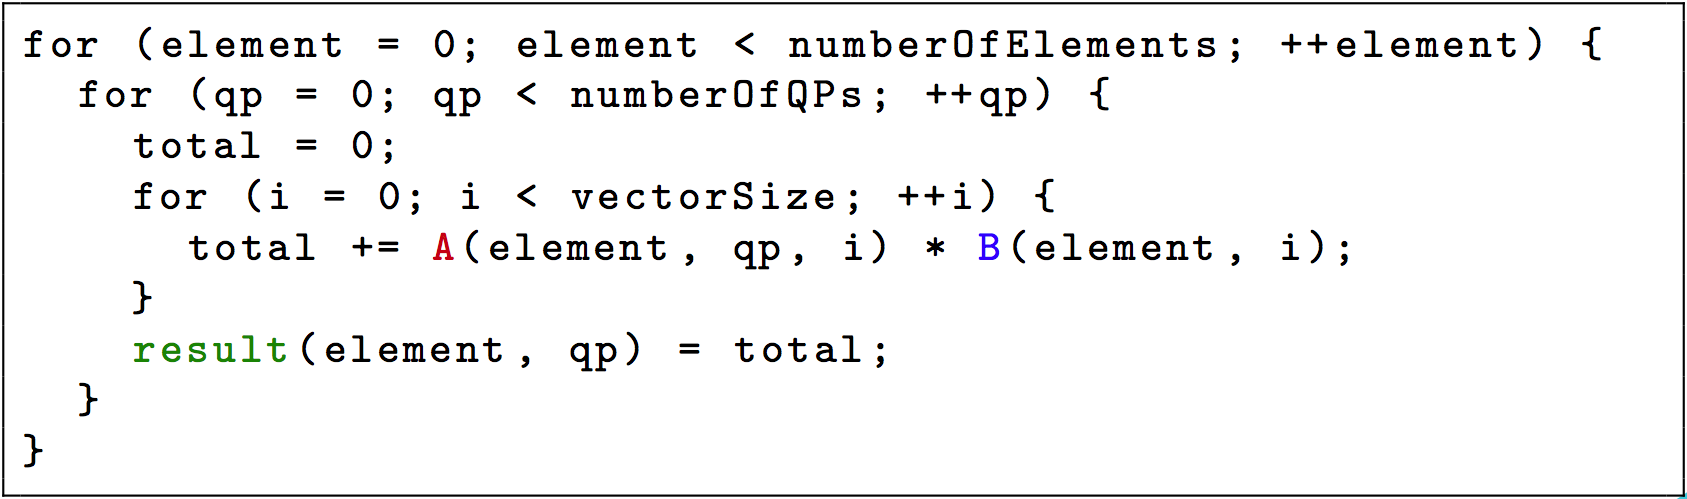
\includegraphics[width=1.00\textwidth]{figures/ContractDataFieldScalar_code}
      \end{center}
    \column{.45\textwidth}
      \begin{center}
        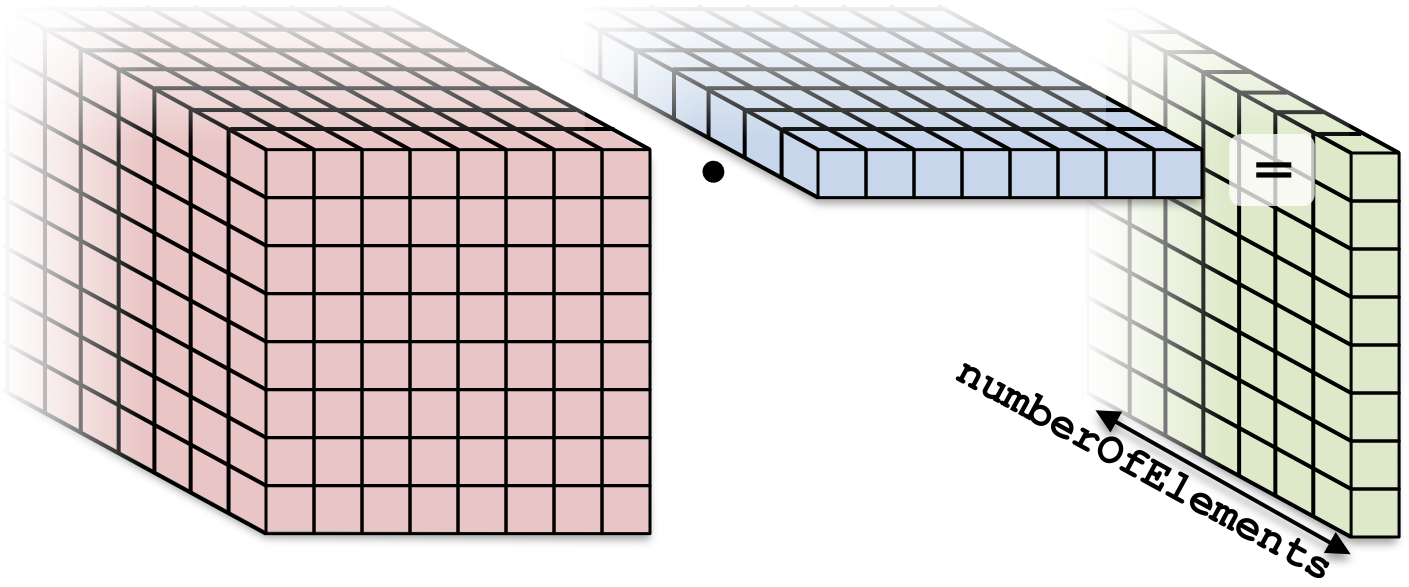
\includegraphics[width=1.00\textwidth]{figures/ContractDataFieldScalar}
      \end{center}
  \end{columns}

  \vspace{10pt}

  \ul{\textbf{Parallelization approaches:}}

  \begin{itemize}[<+->]
    \item{Each thread handles an \texttt{element}. \\
              \hspace{20pt} Threads: \texttt{numberOfElements}}
    \item \tikzmark{infrastructure}{Each thread handles a \texttt{qp}. \\
              \hspace{20pt} Threads: \texttt{numberOfElements * numberOfQPs}}
    \item{Each thread handles an \texttt{i}. \\
              \hspace{20pt} Threads: \texttt{numElements * numQPs * vectorSize}\\
              \hspace{20pt} \emph{Requires a} \texttt{parallel\_reduce}.}
  \end{itemize}

  \tikz[overlay,remember picture]{\draw<+->[draw=black,thick,fill opacity=0.2] ($(infrastructure)+(-0.5,0.4)$) rectangle ($(infrastructure)+(9,-0.6)$);}

\end{frame}

%==========================================================================

\begin{frame}[fragile]{Example: contractDataFieldScalar (4)}

  \begin{columns}[t,onlytextwidth]
    \column{.55\textwidth}
      \begin{center}
        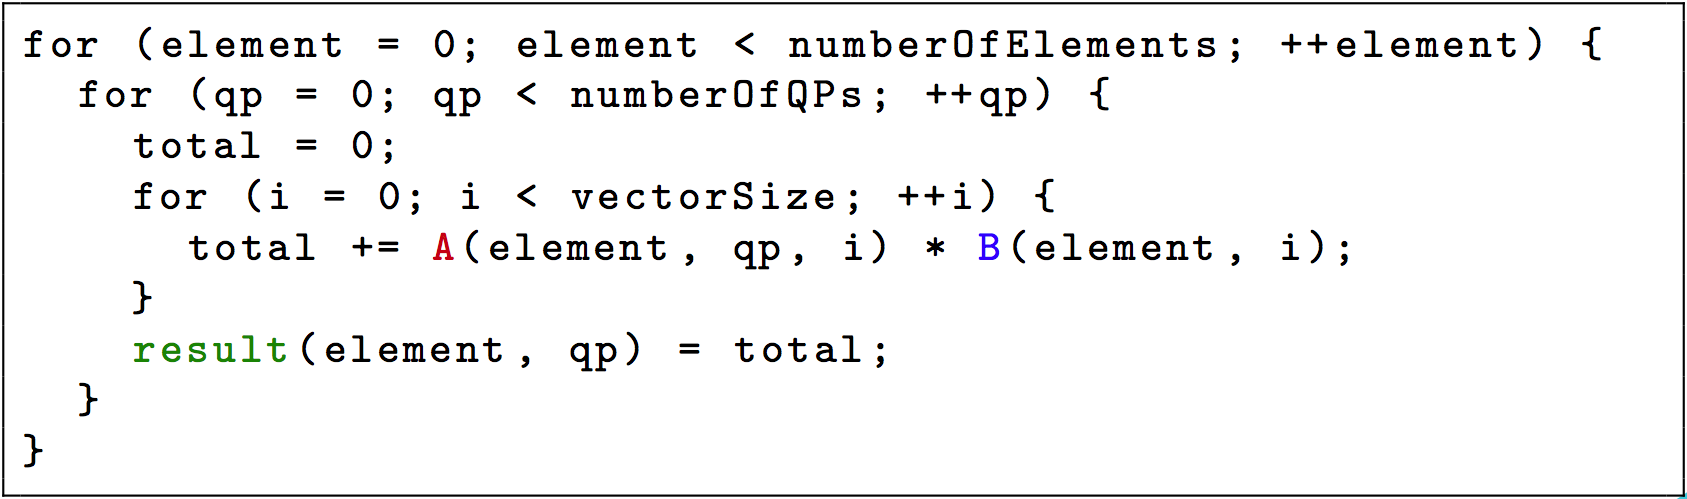
\includegraphics[width=1.00\textwidth]{figures/ContractDataFieldScalar_code}
      \end{center}
    \column{.45\textwidth}
      \begin{center}
        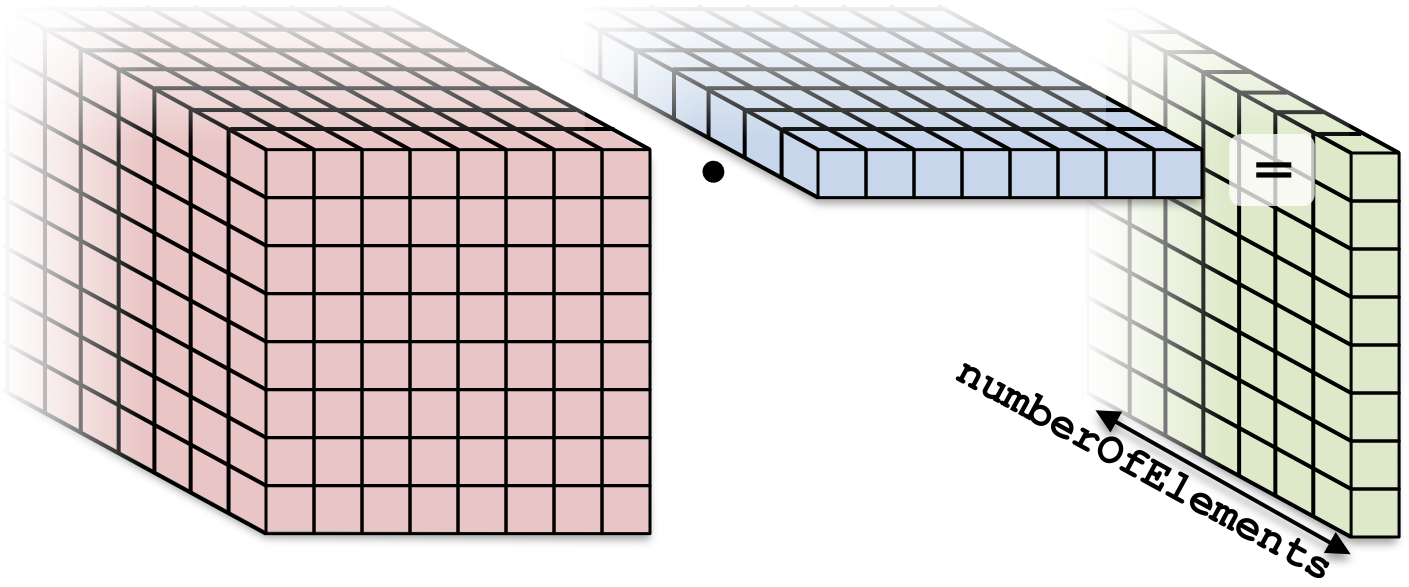
\includegraphics[width=1.00\textwidth]{figures/ContractDataFieldScalar}
      \end{center}
  \end{columns}

  \vspace{10pt}

  \ul{\textbf{Flat kernel:} Each thread handles a quadrature point}

  \begin{code}[frame=single, keywords={}]
parallel_for("L",MDRangePolicy<Rank<2>>({0,0},{numE,numQP}),
  KOKKOS_LAMBDA(int element, int qp) {
  @graydouble total = 0;
  for (int i = 0; i < vectorSize; ++i) {
    total += A(element, qp, i) * B(element, i);
  }
  result(element, qp) = total;@gray
}
  \end{code}

\end{frame}


\begin{frame}[fragile]{Example: contractDataFieldScalar (6)}

  \begin{columns}[t,onlytextwidth]
    \column{.55\textwidth}
      \begin{center}
        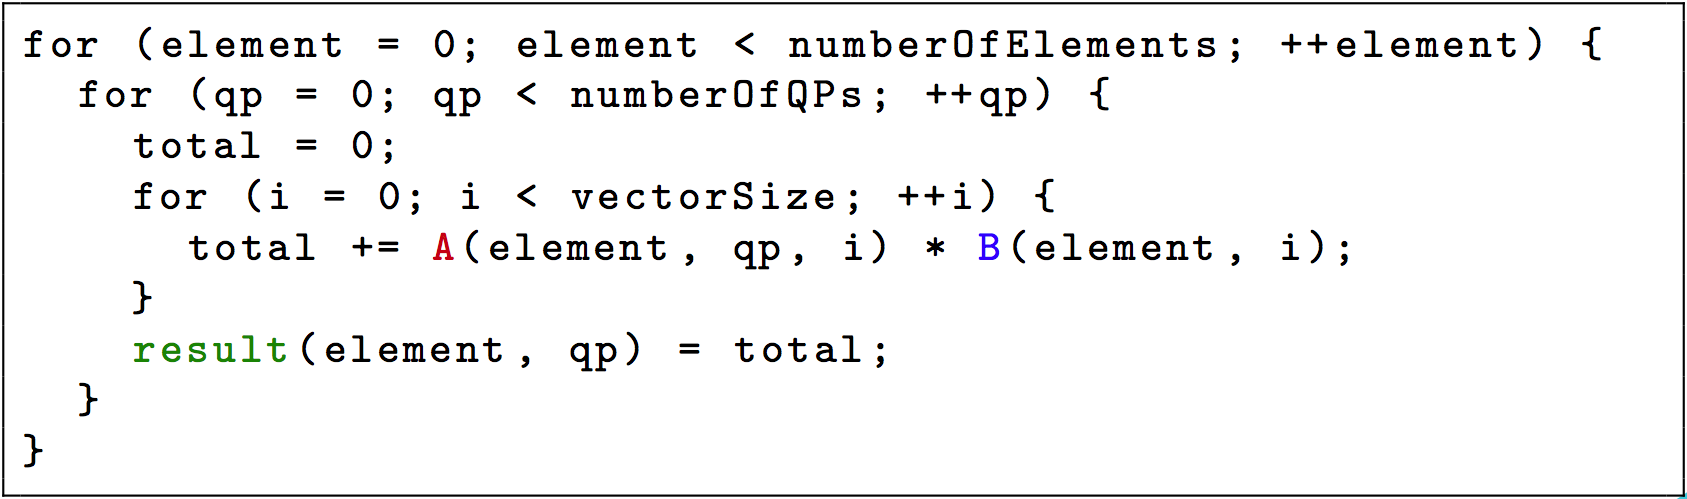
\includegraphics[width=1.00\textwidth]{figures/ContractDataFieldScalar_code}
      \end{center}
    \column{.45\textwidth}
      \begin{center}
        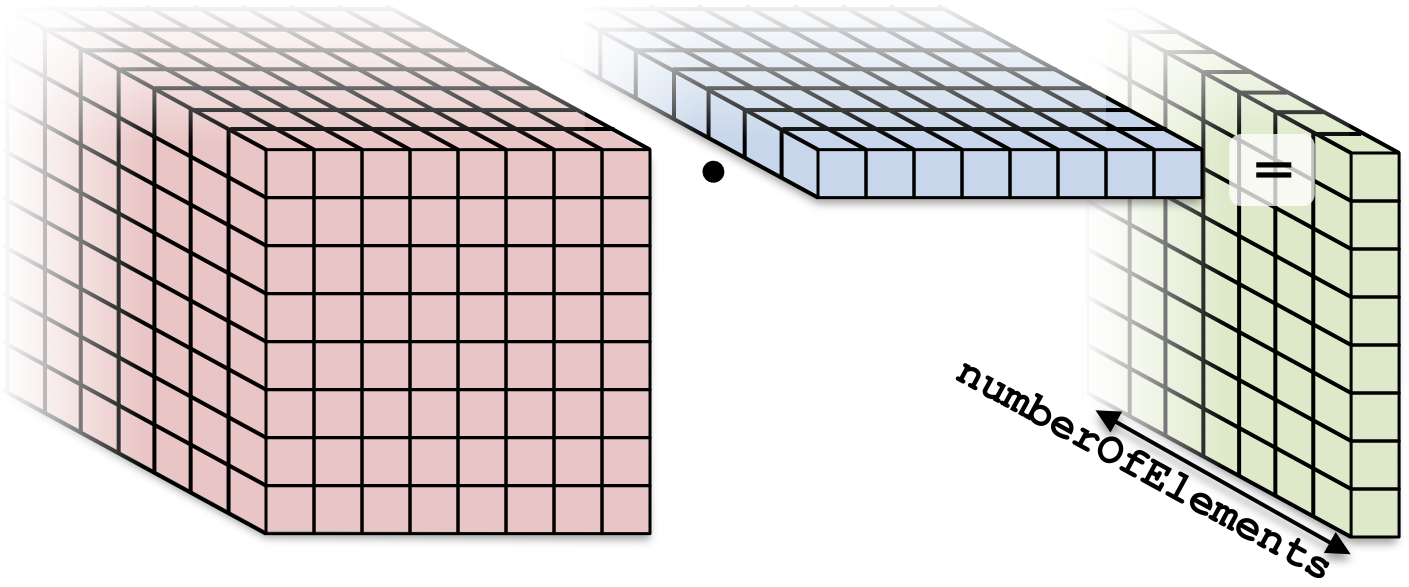
\includegraphics[width=1.00\textwidth]{figures/ContractDataFieldScalar}
      \end{center}
  \end{columns}

  \vspace{0pt}

  \ul{\textbf{Teams kernel:} Each team handles an element}

  \begin{code}[frame=single, keywords={}]
operator()(member_type teamMember) {
  int element = teamMember.league_rank();
  parallel_for(
    TeamThreadRange(teamMember, numberOfQPs),
    [=] (int qp) {
      @graydouble total = 0;
      for (int i = 0; i < vectorSize; ++i) {
        total += A(element, qp, i) * B(element, i);
      }
      result(element, qp) = total;@gray
    });
}
  \end{code}

  \begin{textblock*}{0.50\textwidth}(0.70\textwidth,0.865\textheight)
\only<2->{No real advantage (yet)}
  \end{textblock*}
\end{frame}

%==========================================================================

\begin{frame}[fragile]{Scratch memory (0)}

  Each team has access to a ``scratch pad''.

  \vspace{-10pt}

  \begin{center}
    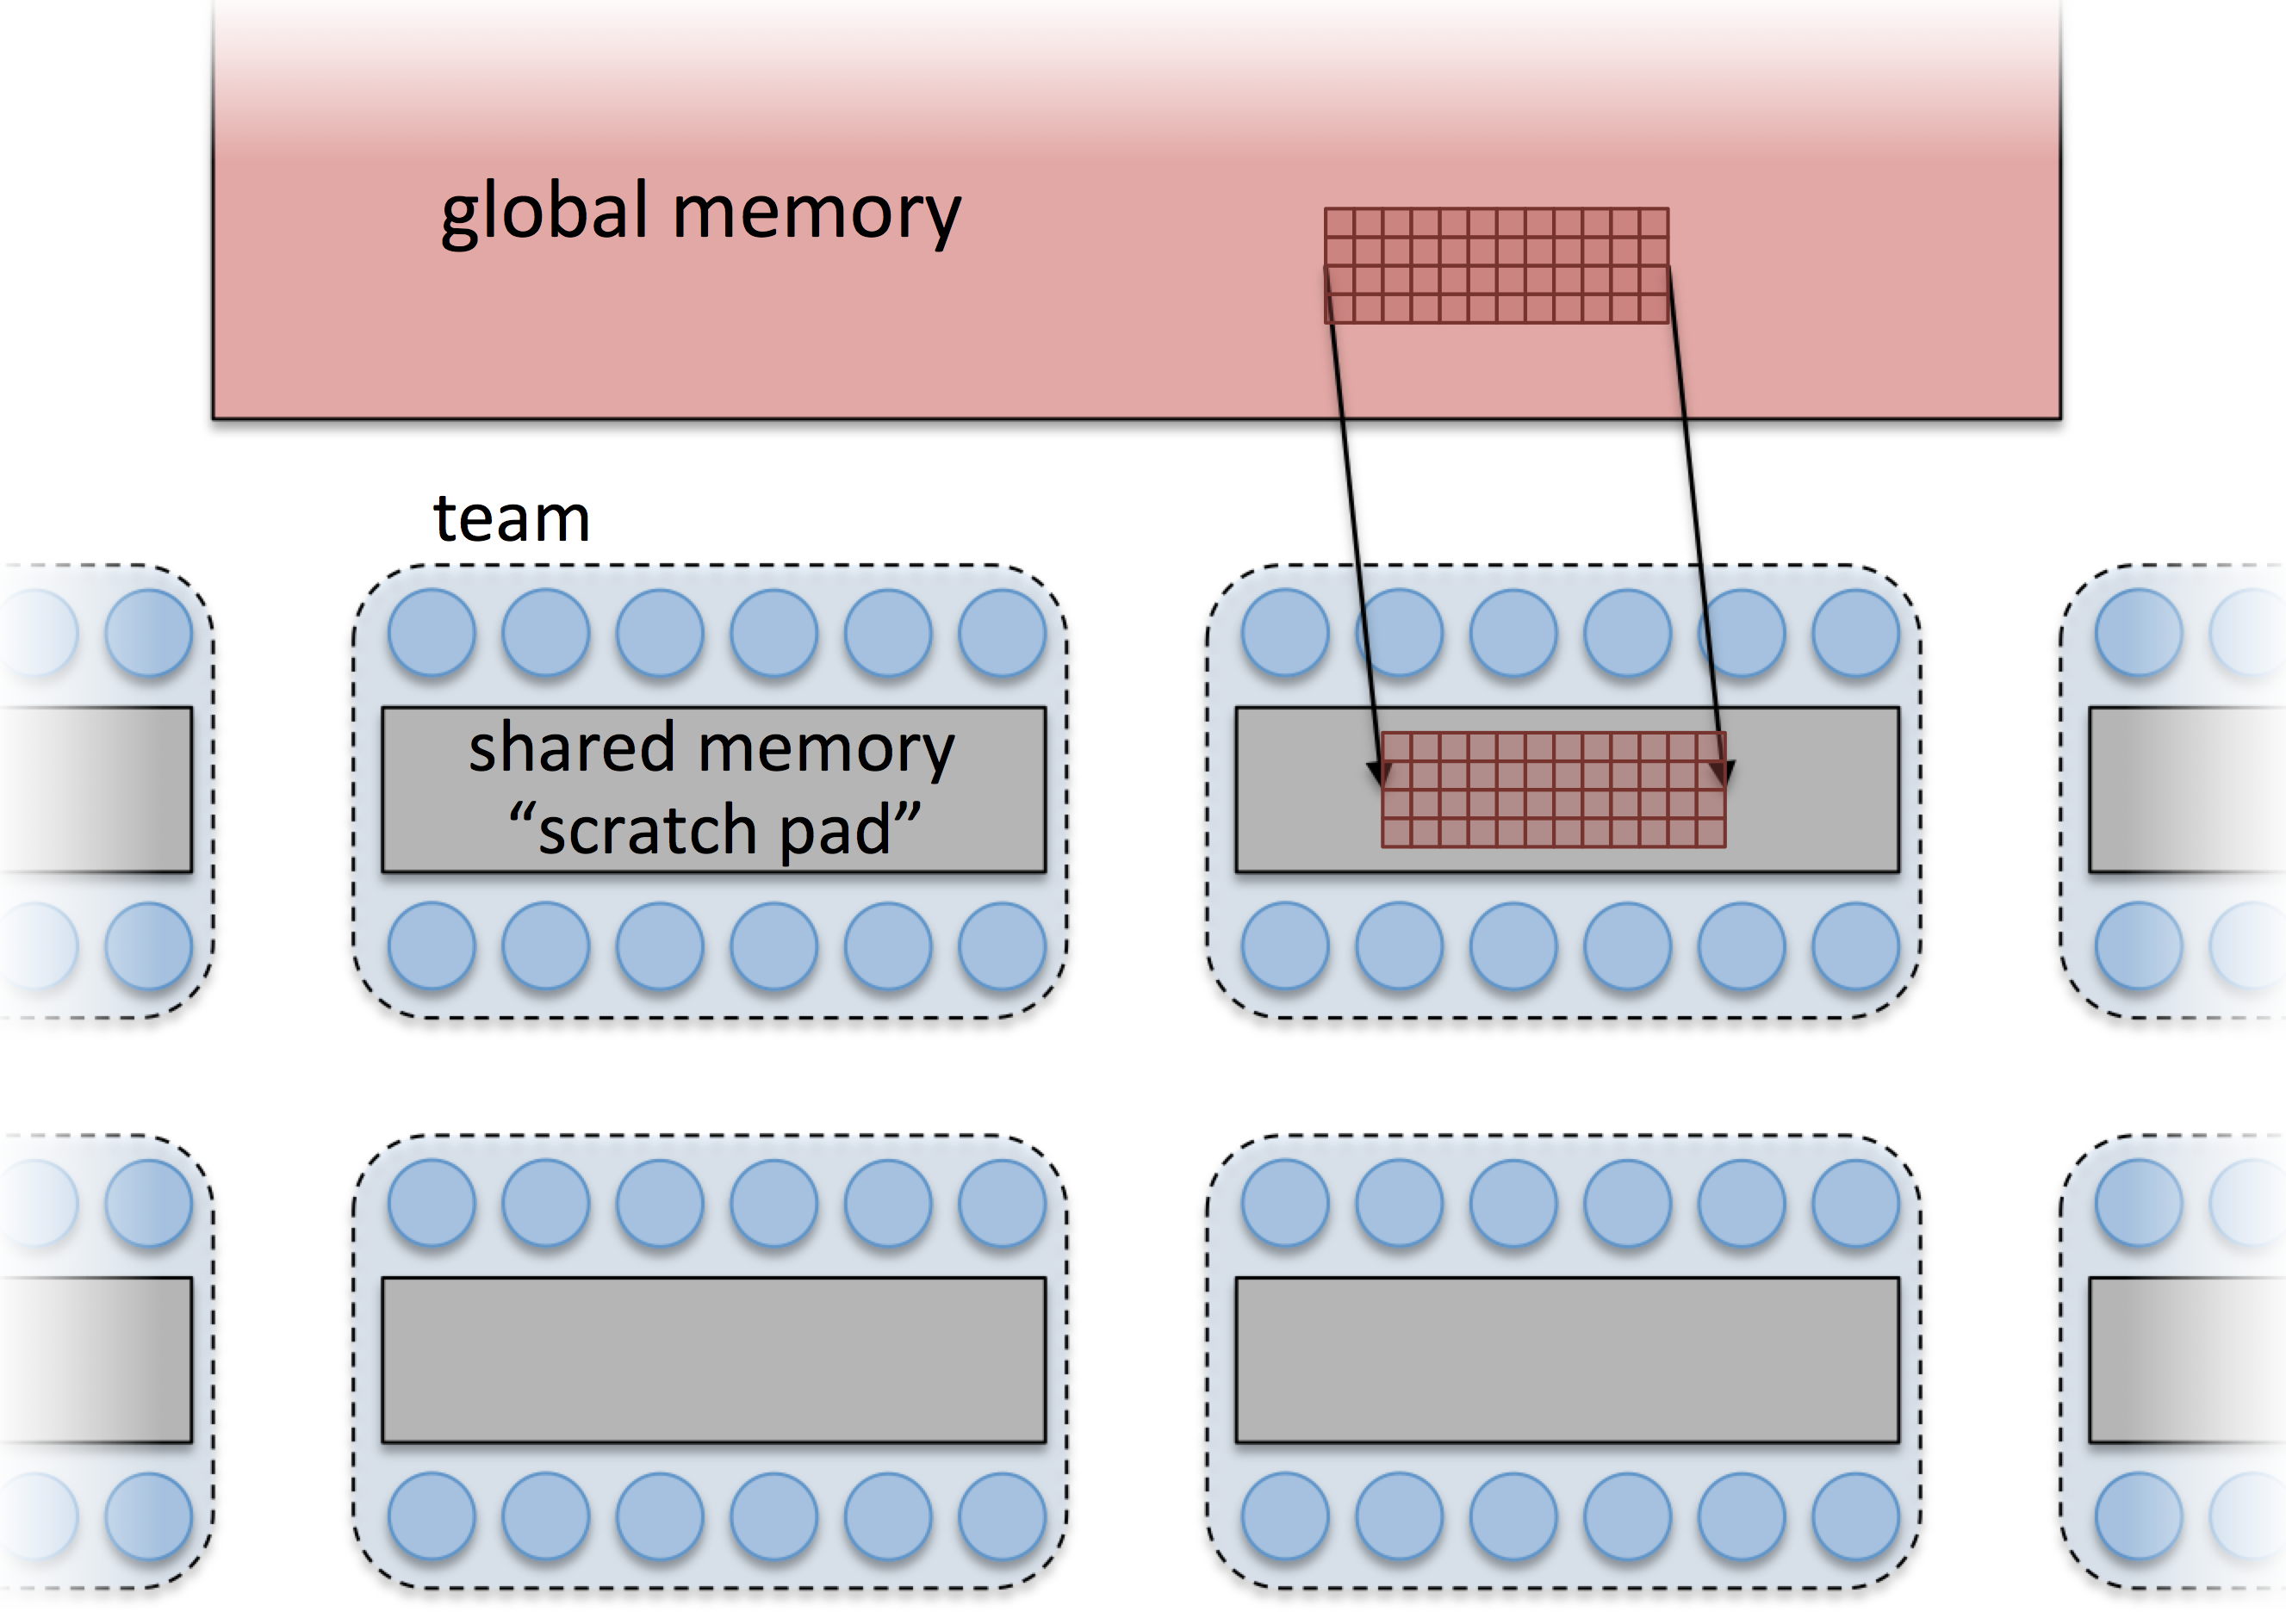
\includegraphics[width=0.90\textwidth]{figures/Hierarchical_sharedMemory}
  \end{center}

\end{frame}

%==========================================================================

\begin{frame}[fragile]{Scratch memory (1)}

  \textbf{Scratch memory (scratch pad) as manual cache:}

  \begin{itemize}
    \item{Accessing data in (level 0) scratch memory is (usually) \textbf{much faster} than global memory.}
    \item{\textbf{GPUs} have separate, dedicated, small, low-latency scratch memories (\emph{NOT subject to coalescing requirements}).}
    \item{\textbf{CPUs} don't have special hardware, but programming with scratch memory results in cache-aware memory access patterns.}
    \item{Roughly, it's like a \emph{user-managed} L1 cache.}
  \end{itemize}

  \pause

  \begin{block}{Important concept}
    When members of a team read the same data multiple times, it's better to load the data into scratch memory and read from there.
  \end{block}

\end{frame}

%==========================================================================

\begin{frame}[fragile]{Scratch memory (2)}

  \textbf{Scratch memory for temporary per work-item storage:}

  \begin{itemize}
    \item{Scenario: Algorithm requires temporary workspace of size W.}
    \item{\textbf{Without scratch memory:} pre-allocate space for N work-items of size N x W.}
    \item{\textbf{With scratch memory:} Kokkos pre-allocates space for each Team or Thread of size T x W.}
    \item{\texttt{PerThread} and \texttt{PerTeam} scratch can be used concurrently.}
    \item{Level 0 and Level 1 scratch memory can be used concurrently.}
  \end{itemize}

  \pause

  \begin{block}{Important concept}
    If an algorithm requires temporary workspace for each work-item, then use Kokkos' scratch memory.
  \end{block}

\end{frame}

%==========================================================================

\begin{frame}[fragile]{Scratch memory (3)}

  To use scratch memory, you need to:
  \begin{enumerate}
    \item{\textbf{Tell Kokkos how much} scratch memory you'll need.}
    \item{\textbf{Make} scratch memory \textbf{views} inside your kernels.}
  \end{enumerate}

  \pause
  \begin{code}
  TeamPolicy<ExecutionSpace> policy(numberOfTeams, teamSize);

  // Define a scratch memory view type
  using ScratchPadView =
      View<double*,@darkredExecutionSpace::scratch_memory_space@darkred>;
  // Compute how much scratch memory (in bytes) is needed
  size_t bytes = ScratchPadView::shmem_size(vectorSize);

  // Tell the policy how much scratch memory is needed
  int level = 0;
  parallel_for(policy.set_scratch_size(level, PerTeam(bytes)),
    KOKKOS_LAMBDA (const member_type& teamMember) {

      // Create a view from the pre-existing scratch memory
      ScratchPadView scratch(teamMember.@darkredteam_scratch(level)@darkred,
                             vectorSize);
  });
  \end{code}
\end{frame}

%==========================================================================

\begin{frame}[fragile]{Example: contractDataFieldScalar (7)}

  \ul{\textbf{Kernel outline for teams with scratch memory:}}

  \begin{code}[keywords={}]
@grayoperator()(member_type teamMember) {@gray
  ScratchPadView @bluescratch@blue(teamMember.team_scratch(0),
                         vectorSize);
  // TODO: load slice of B into scratch

  @grayparallel_for(
    TeamThreadRange(teamMember, numberOfQPs),
    [=] (int qp) {
      double total = 0;
      for (int i = 0; i < vectorSize; ++i) {@gray
        // total += A(element, qp, i) * B(element, i);
        total += A(element, qp, i) * @bluescratch@blue(i);
      @gray}
      result(element, qp) = total;
    });
}@gray
  \end{code}

  \begin{tikzpicture}[remember picture, overlay]
    \node [shift={(-5.6cm,0.85cm)}]  at (current page.south east)
      {%
      \begin{tikzpicture}[remember picture, overlay]
        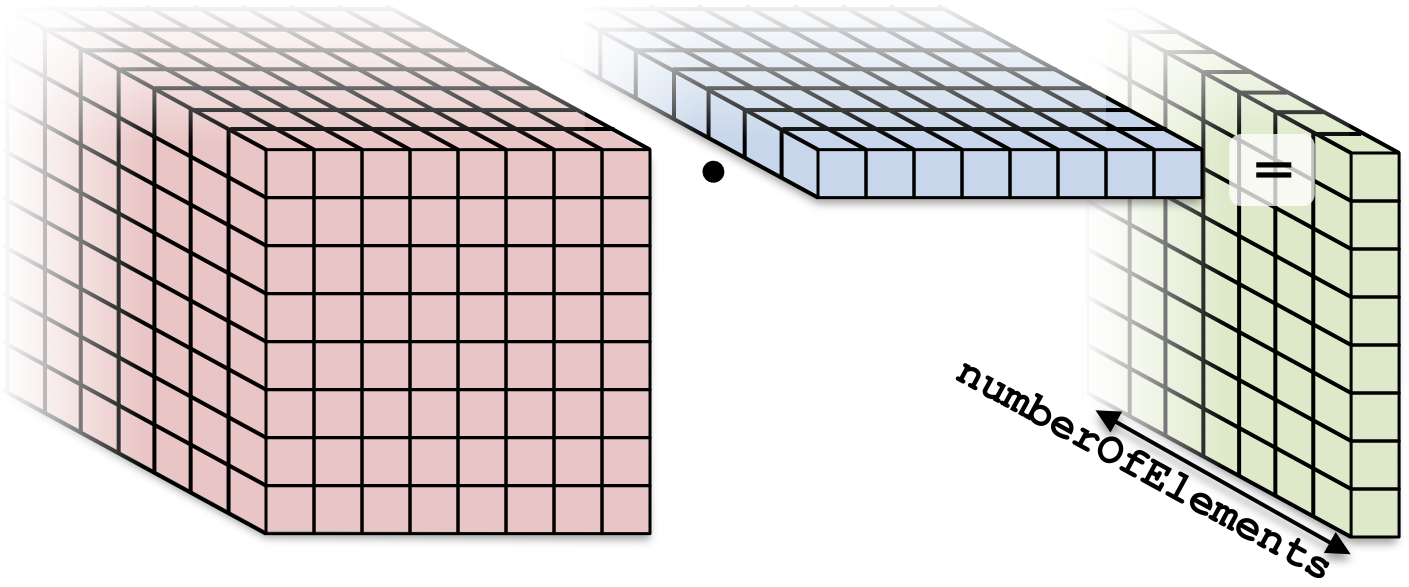
\includegraphics[width=0.45\textwidth]{figures/ContractDataFieldScalar}
      \end{tikzpicture}
      };
  \end{tikzpicture}

\end{frame}

%==========================================================================

\begin{frame}[fragile]{Example: contractDataFieldScalar (8)}

  \begin{tikzpicture}[remember picture, overlay]
    \node [shift={(-5.6cm,0.85cm)}]  at (current page.south east)
      {%
      \begin{tikzpicture}[remember picture, overlay]
        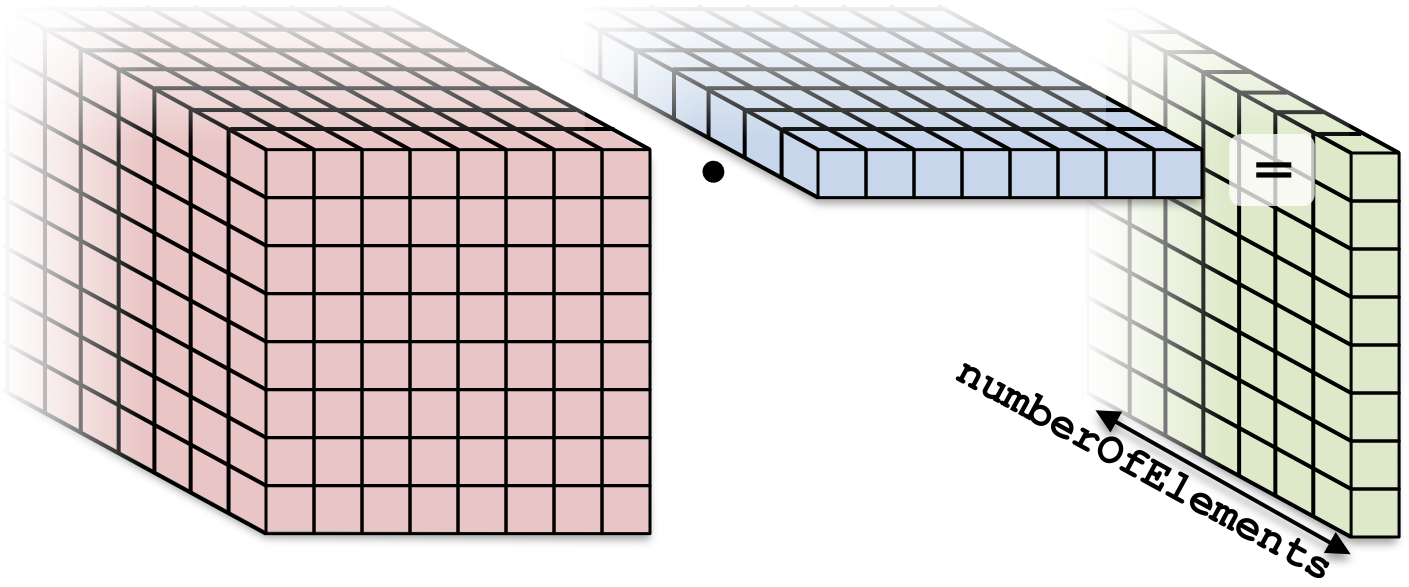
\includegraphics[width=0.45\textwidth]{figures/ContractDataFieldScalar}
      \end{tikzpicture}
      };
  \end{tikzpicture}

  \ul{\textbf{How to populate the scratch memory?}}

  \begin{itemize}
    \item<1->\only<1>{One thread loads it all?}\only<2->{\st{One thread loads it all?} \hspace{10pt} {\color{red}Serial}}

  \begin{code}[keywords={}]
if (teamMember.team_rank() == 0) {
  for (int i = 0; i < vectorSize; ++i) {
    @bluescratch@blue(i) = B(element, i);
  }
}
  \end{code}

    \item<2->\only<2>{Each thread loads one entry?}\only<3->{\st{Each thread loads one entry?} \hspace{10pt} {\color{red}\texttt{teamSize $\neq$ vectorSize}}}

  \only<1>{\hspace{0pt}}

  \onslide<2->

  \begin{code}[keywords={}]
@bluescratch@blue(team_rank) = B(element, team_rank);
  \end{code}

    \item<3->\tikzmark{left}\only<3-4>{\texttt{TeamVectorRange}}\tikzmark{right}

  \only<1-2>{\hspace{0pt}}

  \onslide<3->

  \begin{code}[keywords={}]
parallel_for(
  TeamVectorRange(teamMember, vectorSize),
  [=] (int i) {
    @bluescratch@blue(i) = B(element, i);
  });
  \end{code}

  \end{itemize}

  \only<4>{\DrawBoxWideBlack*[thick]}

  \vspace{50pt}

\end{frame}

%==========================================================================

\begin{frame}[fragile]{Example: contractDataFieldScalar (9)}

  \ul{\textbf{(incomplete) Kernel for teams with scratch memory:}}

  \begin{code}[keywords={}]
@grayoperator()(member_type teamMember) {@gray
  ScratchPadView @bluescratch@blue(...);

  @grayparallel_for(TeamVectorRange(teamMember, vectorSize),
    [=] (int i) {@gray
      @bluescratch@blue(i) = B(element, i);
    @gray});@gray
  // TODO: fix a problem at this location

  @grayparallel_for(TeamThreadRange(teamMember, numberOfQPs),
    [=] (int qp) {
      double total = 0;
      for (int i = 0; i < vectorSize; ++i) {@gray
        total += A(element, qp, i) * @bluescratch@blue(i);
      @gray}
      result(element, qp) = total;
    });
}@gray
  \end{code}

  \pause
  \vspace{-5pt}

  {\color{red}Problem}: threads may start to use {\color{blue}\texttt{scratch}} before all threads are done loading.

\end{frame}

%==========================================================================

\begin{frame}[fragile]{Example: contractDataFieldScalar (10)}

  \ul{\textbf{Kernel for teams with scratch memory:}}

  \begin{code}[keywords={}]
@grayoperator()(member_type teamMember) {@gray
  ScratchPadView @bluescratch@blue(...);

  @grayparallel_for(TeamVectorRange(teamMember, vectorSize),
    [=] (int i) {@gray
      @bluescratch@blue(i) = B(element, i);
    @gray});@gray
  @boldteamMember.team_barrier();@bold

  @grayparallel_for(TeamThreadRange(teamMember, numberOfQPs),
    [=] (int qp) {
      double total = 0;
      for (int i = 0; i < vectorSize; ++i) {@gray
        total += A(element, qp, i) * @bluescratch@blue(i);
      @gray}
      result(element, qp) = total;
    });
}@gray
  \end{code}

  \vspace{19pt}

  \begin{tikzpicture}[remember picture, overlay]
    \node [shift={(-5.6cm,0.85cm)}]  at (current page.south east)
      {%
      \begin{tikzpicture}[remember picture, overlay]
        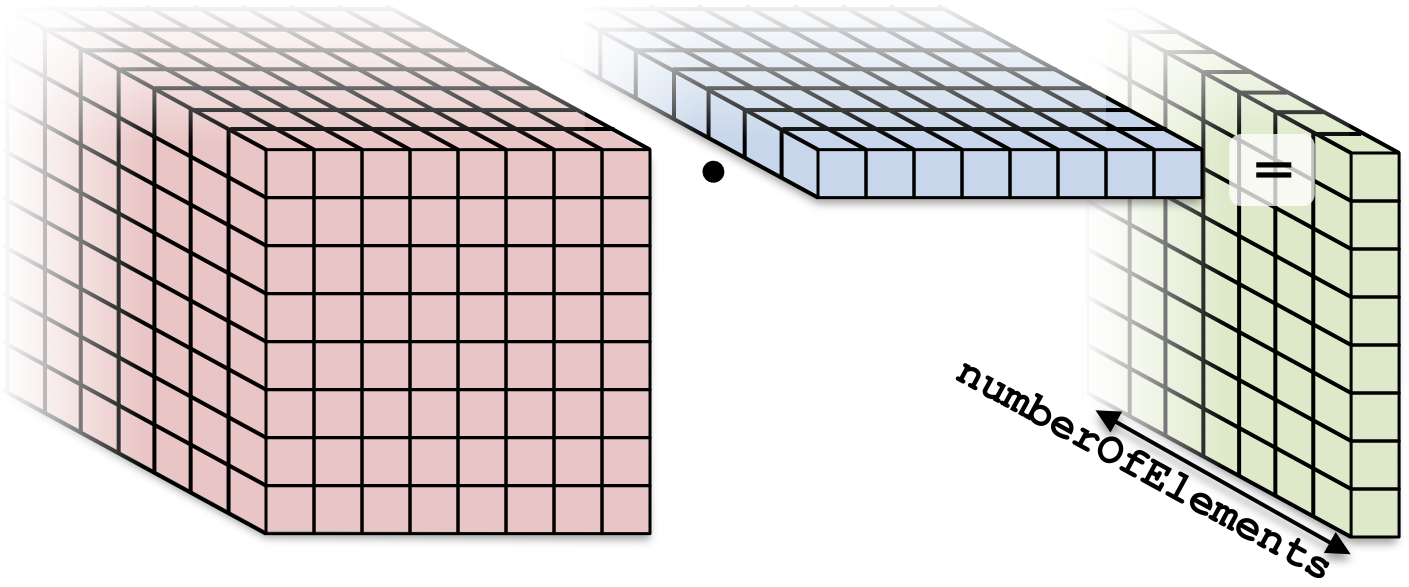
\includegraphics[width=0.50\textwidth]{figures/ContractDataFieldScalar}
      \end{tikzpicture}
      };
  \end{tikzpicture}

\end{frame}

%==========================================================================

\begin{frame}[fragile]{Exercise: Scratch Memory}
Use Scratch Memory to explicitly cache the x-vector for each element.

  \vspace{10pt}

  \textbf{Details}:
  \begin{small}
  \begin{itemize}
\item Location: \ExerciseDirectory{team\_scratch\_memory}
\item Create a scratch view
\item Fill the scratch view in parallel using a TeamVectorRange
\end{itemize}
  \end{small}

\ul{\textbf{Things to try:}}
  \begin{small}
  \begin{itemize}
  \item Vary problem size and number of rows (-S ...; -N ...)
  \item Compare behavior with Exercise 6
  \item Compare behavior of CPU vs GPU
  \end{itemize}
  \end{small}
\end{frame}

%==========================================================================

\begin{frame}[fragile]{Exercise: Scratch Memory}

  %\vspace{-10pt}

    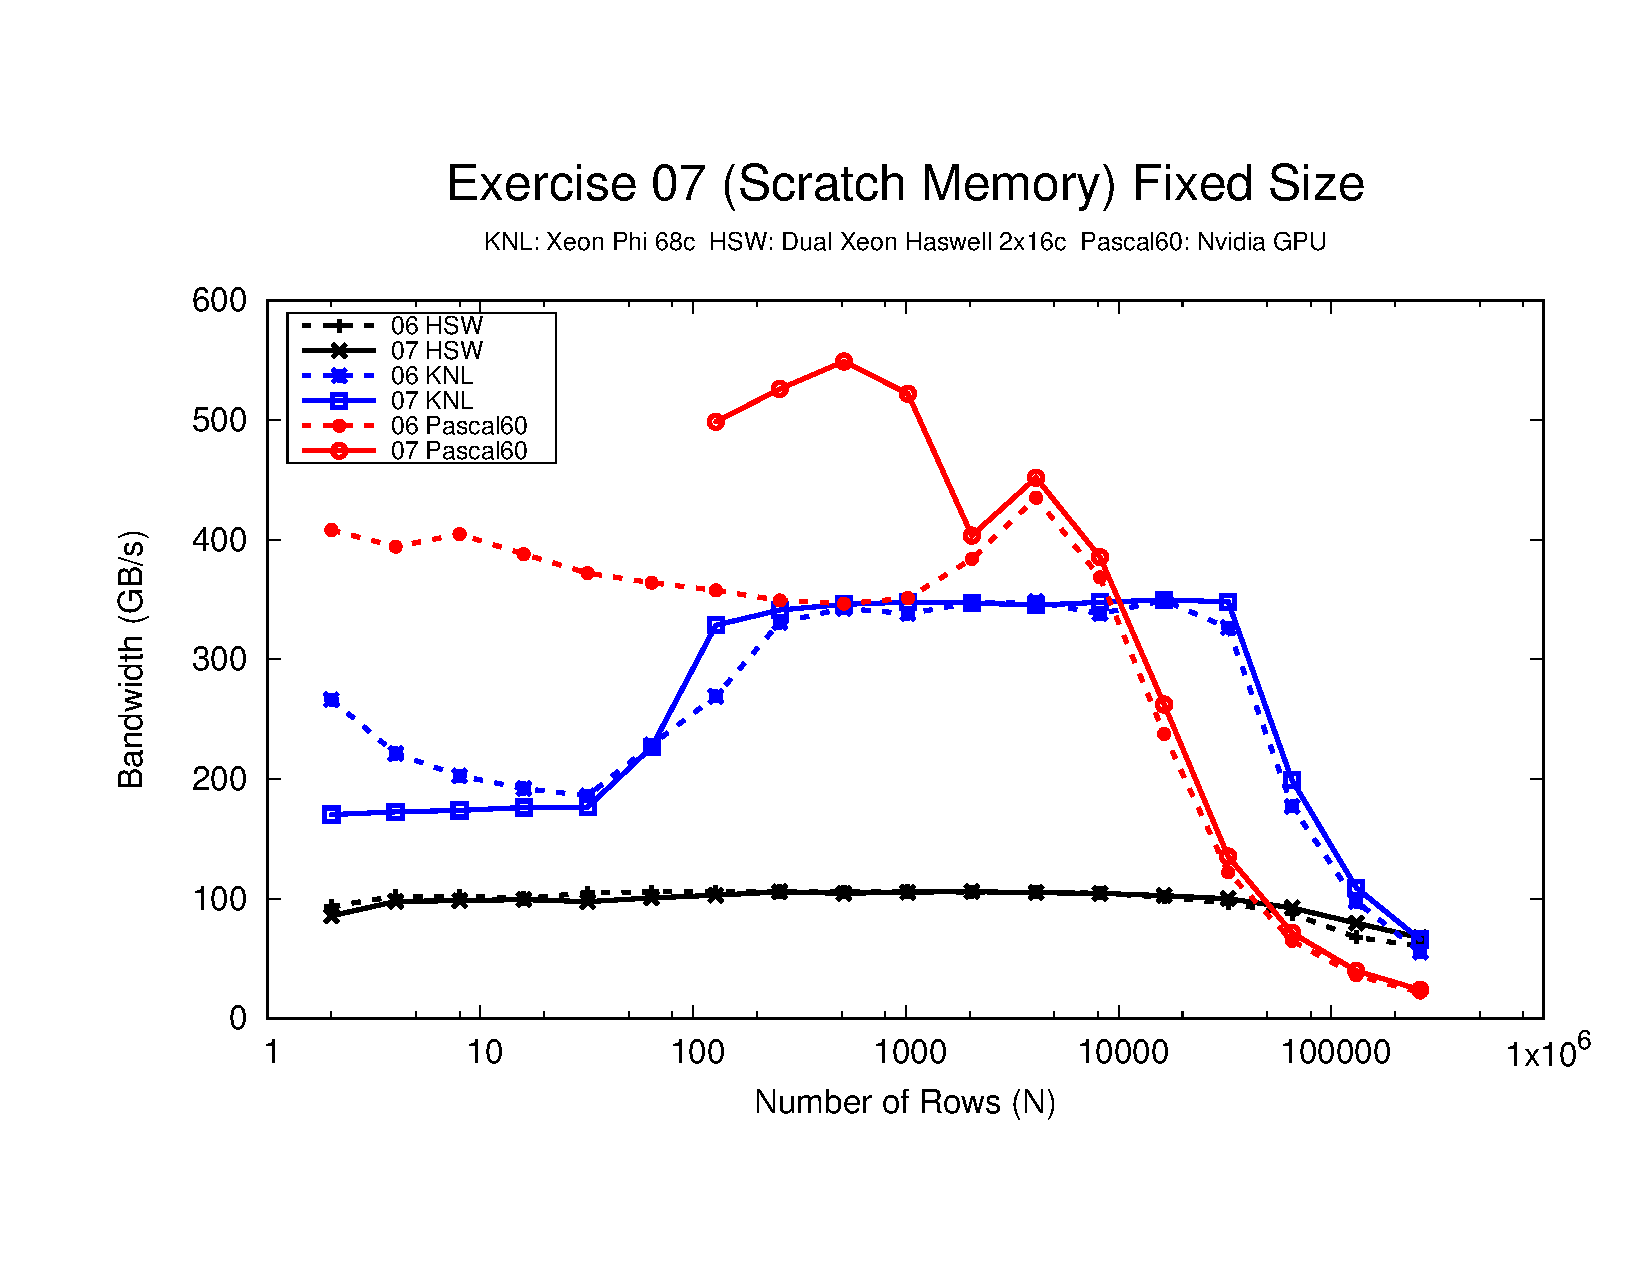
\includegraphics[viewport=1.25in 3.0in 10in 6in, width=0.95\textwidth]{figures/Exercise07-Performance.pdf}

  \vspace{-15pt}

\end{frame}

%==========================================================================

\begin{frame}[fragile]{Scratch Memory: API Details}
Allocating scratch in different levels:
  \begin{code}[keywords=level]
  int level = 1; // valid values 0,1
  policy.set_scratch_size(level,PerTeam(bytes));
  \end{code}

\pause

Using PerThread, PerTeam or both:
  \begin{code}[keywords={PerTeam,PerThread}]
  policy.set_scratch_size(level,PerTeam(bytes));
  policy.set_scratch_size(level,PerThread(bytes));
  policy.set_scratch_size(level,PerTeam(bytes1),
                                PerThread(bytes2));
  \end{code}

\pause

Using both levels of scratch:
  \begin{code}[keywords={PerTeam,PerThread}]
  policy.set_scratch_size(0,PerTeam(bytes0))
        .set_scratch_size(1,PerThread(bytes1));
  \end{code}

Note: \texttt{set\_scratch\_size()} returns a new policy instance, it doesn't modify the existing one.
\end{frame}

%==========================================================================

\begin{frame}{Section Summary}

  \begin{itemize}
    \item{\textbf{Scratch Memory} can be use with the \texttt{TeamPolicy} to provide thread or team \textbf{private} memory.}
    \item{Usecase: per work-item temporary storage or manual caching.}
    \item{Scratch memory exposes on-chip user managed caches (e.g. on NVIDIA GPUs)}
    \item{The size must be determined before launching a kernel.}
    \item{Two levels are available: large/slow and small/fast.}
  \end{itemize}

\end{frame}
